\documentclass[12pt, a4paper]{article}

% ── Packages ──────────────────────────────────────────────────────────────────
\usepackage[a4paper, margin=2.5cm]{geometry}
\usepackage{graphicx}
\usepackage{float}
\usepackage{amsmath}
\usepackage{amssymb}
\usepackage{xcolor}
\usepackage{mdframed}
\usepackage{parskip}
\usepackage{enumitem}
\usepackage{titlesec}
\usepackage{booktabs}
\usepackage{hyperref}
\usepackage[T1]{fontenc}
\usepackage[colorinlistoftodos]{todonotes}
\usepackage{listings}
\usepackage{courier}

% ── Graphics path ─────────────────────────────────────────────────────────────
\graphicspath{{../../Images_for_latex/Lecture_5/}}

% ── Colours ───────────────────────────────────────────────────────────────────
\definecolor{keyblue}{RGB}{30, 80, 160}
\definecolor{keybluebg}{RGB}{220, 235, 255}
\definecolor{noteorange}{RGB}{200, 100, 0}
\definecolor{noteorangebg}{RGB}{255, 240, 215}
\definecolor{warnred}{RGB}{180, 30, 30}
\definecolor{warnredbg}{RGB}{255, 220, 220}
\definecolor{defgreen}{RGB}{20, 110, 50}
\definecolor{defgreenbg}{RGB}{215, 245, 225}
\definecolor{headernavy}{RGB}{25, 35, 90}
\definecolor{codegray}{RGB}{245, 245, 245}
\definecolor{codecomment}{RGB}{100, 100, 100}

% ── Box environments ──────────────────────────────────────────────────────────
\newmdenv[linecolor=keyblue, backgroundcolor=keybluebg, linewidth=1.5pt,
  leftline=true, rightline=false, topline=false, bottomline=false,
  innerleftmargin=10pt, innerrightmargin=8pt,
  innertopmargin=6pt, innerbottommargin=6pt,
  skipabove=8pt, skipbelow=8pt]{keybox}

\newmdenv[linecolor=noteorange, backgroundcolor=noteorangebg, linewidth=1.5pt,
  leftline=true, rightline=false, topline=false, bottomline=false,
  innerleftmargin=10pt, innerrightmargin=8pt,
  innertopmargin=6pt, innerbottommargin=6pt,
  skipabove=8pt, skipbelow=8pt]{notebox}

\newmdenv[linecolor=warnred, backgroundcolor=warnredbg, linewidth=1.5pt,
  leftline=true, rightline=false, topline=false, bottomline=false,
  innerleftmargin=10pt, innerrightmargin=8pt,
  innertopmargin=6pt, innerbottommargin=6pt,
  skipabove=8pt, skipbelow=8pt]{warnbox}

\newmdenv[linecolor=defgreen, backgroundcolor=defgreenbg, linewidth=1.5pt,
  leftline=true, rightline=false, topline=false, bottomline=false,
  innerleftmargin=10pt, innerrightmargin=8pt,
  innertopmargin=6pt, innerbottommargin=6pt,
  skipabove=8pt, skipbelow=8pt]{defbox}

% ── Section formatting ────────────────────────────────────────────────────────
\titleformat{\section}[block]{\large\bfseries\color{headernavy}}{}{0pt}{}
  [\vspace{2pt}\rule{\linewidth}{0.8pt}\vspace{4pt}]
\titleformat{\subsection}[block]{\normalsize\bfseries\color{keyblue}}{}{0pt}{}

% ── Inline label commands ─────────────────────────────────────────────────────
\newcommand{\keynote}[1]{\textbf{\color{keyblue}#1}}
\newcommand{\warn}[1]{\textbf{\color{warnred}#1}}

% ── Code listing style ────────────────────────────────────────────────────────
\lstset{
  language=Python,
  basicstyle=\footnotesize\ttfamily,
  backgroundcolor=\color{codegray},
  commentstyle=\color{codecomment}\itshape,
  keywordstyle=\color{keyblue}\bfseries,
  stringstyle=\color{defgreen},
  breaklines=true,
  frame=single,
  framerule=0.5pt,
  rulecolor=\color{keyblue!40},
  numbers=left,
  numberstyle=\tiny\color{codecomment},
  numbersep=6pt,
  xleftmargin=12pt,
  showstringspaces=false,
}

% ── Document ──────────────────────────────────────────────────────────────────
\begin{document}

% ── Title ─────────────────────────────────────────────────────────────────────
\begin{center}
  {\LARGE\bfseries\color{headernavy} Sensors \& Systems --- Exercise Notes}\\[4pt]
  {\large Lecture 5 \quad Exercise 1: 1D Kalman Filter for IMU}\\[2pt]
  {\normalsize Jan Bendtsen, Torben Knudsen \quad|\quad Electronic Systems, 8th Semester}
\end{center}

\vspace{4pt}
\hrule height 1.2pt
\vspace{12pt}

\section*{Exercise Statement}

Implement the Kalman filter for the 1D IMU (perfect model/estimator match)
shown in the slides with:
\[
  \phi = 0.9, \quad
  \sigma_{w_a} = \sigma_{w_b} = \sigma_\nu = 0.1, \quad
  b = -0.2, \quad
  T_s = 0.001
\]
Replicate the figures on Slide~25 (see Figure~\ref{fig:slide25ref}).

\begin{figure}[H]
  \centering
  
\includegraphics[width=0.7\linewidth]{slide-25.jpg}
  \caption{Slide~25 reference result.
           \textbf{Blue} = true signal; \textbf{Red} = KF estimate.
           From top to bottom: position $x_k$, velocity $v_k$,
           acceleration $a_k$, bias $b_k$.
           Time axis $t = 0\ldots50$\,s.}
  \label{fig:slide25ref}
\end{figure}

\begin{notebox}
  \textbf{A full IMU has three sensor types - this exercise uses only one.}\\
  The gyroscope and magnetometer are essential for 3-D attitude (roll,
  pitch, yaw) estimation.
  That problem is nonlinear (trigonometric functions of the current
  orientation appear in the equations), which forces us to use the
  Extended or Unscented KF.
  In this 1-D exercise the system is linear throughout --- the standard
  linear KF applies directly.
\end{notebox}

\clearpage
\subsection*{Stochastic errors --- tracked by the Kalman filter}
\begin{defbox}
  \textbf{White noise} $\boldsymbol{\nu}$\\
  Origin: thermo-mechanical fluctuations inside the MEMS structure
  (Brownian motion of the proof mass).\\
  Model: $\nu_k \sim \mathcal{N}(0,\,\sigma_\nu^2)$, independent
  sample to sample.

  \textbf{Key property:} each sample is equally likely to be above
  or below the true value.
  The mean is zero \emph{and} stays zero at every instant --- because
  consecutive samples are independent, there is no accumulation.
\end{defbox}

\begin{defbox}
  \textbf{Bias random walk} $\boldsymbol{\epsilon}$\\
  Origin: \textbf{flicker noise} ($1/f$) in the analogue readout --- slow fluctuations that drift the DC operating point.
  Model: $b_{k+1} = b_k + \sigma_{w_b}\,\bar{w}_{b,k}$,\quad $\bar{w}_{b,k} \sim \mathcal{N}(0,1)$.\\[4pt]
  \textbf{Key property:} each increment is zero-mean, but the bias accumulates all past increments, so its variance grows as $\sigma_{w_b}^2 k$ --- it wanders without bound and cannot be calibrated away.\\[4pt]
  In the exercise: $\sigma_{w_b} = 0.1$.
\end{defbox}
\subsection*{Deterministic errors --- remove by calibration}

\textbf{Accelerometer:}
\[
  K_a\tilde{\mathbf{a}}
    = (I + S_a + M_a)\,\mathbf{a}
      + \mathbf{b}_a
      + T_a\Delta T
      + \boldsymbol{\nu}_a
      + \boldsymbol{\epsilon}_a
\]

\textbf{Gyroscope:}
\[
  K_g\tilde{\boldsymbol{\omega}}
    = (I + S_g + M_g)\,\boldsymbol{\omega}
      + \mathbf{b}_g
      + G_g\,\mathbf{a}
      + T_g\Delta T
      + \boldsymbol{\nu}_g
      + \boldsymbol{\epsilon}_g
\]
\subsection*{Deterministic errors --- remove by calibration}
\begin{center}
\renewcommand{\arraystretch}{1.4}
\begin{tabular}{p{2.2cm} p{2.8cm} p{8.2cm}}
  \toprule
  \textbf{Symbol} & \textbf{Name} & \textbf{What it does} \\
  \midrule
  $K_a$, $K_g$
    & Sensitivity
    & Overall gain error (volts per m/s$^2$); single scalar per axis. \\
  $S_a$, $S_g$
    & Scale factor distortion
    & Each axis has its own gain error: $x$ reads $1.02\,g$, $y$ reads
      $0.97\,g$.
      Diagonal matrix $\mathrm{diag}(S_x, S_y, S_z)$. \\
  $M_a$, $M_g$
    & Misalignment
    & Axes not exactly $90°$ apart, could be $y$ and $z$ (\textbf{cross-axis coupling}).
      Removed by the \textbf{tumble test} on a precision turntable. \\
  $G_g\mathbf{a}$
    & g-sensitivity (gyro only)
    & Linear acceleration deflects the gyro proof mass, faking a
      rotation signal.
      Significant only in high-$g$ manoeuvres. \\
  $T_a\Delta T$, $T_g\Delta T$
    & Temperature drift
    & MEMS spring stiffness shifts with temperature, moving the bias.
      Corrected at runtime via an on-chip thermometer and lookup table. \\
  \bottomrule
\end{tabular}
\end{center}

\clearpage
\section*{The 4-State Model - Exercise 1}
\subsection*{State vector}
\[
\boldsymbol{\chi}_k = \begin{bmatrix} x_k \\ v_k \\ a_k \\ b_k \end{bmatrix}
\qquad
\begin{aligned}
  &x_k : \text{position [m]}\\
  &v_k : \text{velocity [m/s]}\\
  &a_k : \text{true acceleration [m/s}^2\text{]}\\
  &b_k : \text{accelerometer bias [m/s}^2\text{]}
\end{aligned}
\]
where the bias evolves as a random walk,
\[
  b_{k+1} = b_k + \sigma_{w_b}\,\bar{w}_{b,k}, \qquad \bar{w}_{b,k} \sim \mathcal{N}(0,1),
\]
i.e.\ each step the bias shifts by a zero-mean Gaussian increment with standard deviation $\sigma_{w_b}$.

\subsection*{System matrices}
\textbf{State equation:}
$\boldsymbol{\chi}_{k+1} = \boldsymbol{\Phi}\,\boldsymbol{\chi}_k + Q^{1/2}\bar{\mathbf{w}}_k$
Each row of $\boldsymbol{\Phi}$ encodes one update rule:
\[
\underbrace{
\begin{bmatrix} x_{k+1} \\ v_{k+1} \\ a_{k+1} \\ b_{k+1} \end{bmatrix}
}_{\displaystyle\boldsymbol{\chi}_{k+1}}
=
\underbrace{
\begin{bmatrix}
  1 & T_s & 0    & 0 \\
  0 & 1   & T_s  & 0 \\
  0 & 0   & \phi & 0 \\
  0 & 0   & 0    & 1
\end{bmatrix}
}_{\boldsymbol{\Phi},\;{\scriptsize\text{state transition}}}
\underbrace{
\begin{bmatrix} x_k \\ v_k \\ a_k \\ b_k \end{bmatrix}
}_{\displaystyle\boldsymbol{\chi}_k}
+
\underbrace{
\begin{bmatrix}
  0 & 0 & 0              & 0              \\
  0 & 0 & 0              & 0              \\
  0 & 0 & \sigma_{w_a}^2 & 0              \\
  0 & 0 & 0              & \sigma_{w_b}^2
\end{bmatrix}
}_{Q,\;{\scriptsize\text{process noise}}}^{1/2}
\underbrace{
\begin{bmatrix} 0 \\ 0 \\ \bar{w}_{a,k} \\ \bar{w}_{b,k} \end{bmatrix}
}_{\displaystyle\bar{\mathbf{w}}_k}
\quad
\begin{aligned}
  &\leftarrow x_{k+1} = x_k + T_s v_k \quad \text{(Euler position)}\\
  &\leftarrow v_{k+1} = v_k + T_s a_k \quad \text{(Euler velocity)}\\
  &\leftarrow a_{k+1} = \phi\,a_k + \sigma_{w_a}\bar{w}_{a,k} \quad \text{(AR(1))}\\
  &\leftarrow b_{k+1} = b_k + \sigma_{w_b}\bar{w}_{b,k} \quad \text{(random walk)}
\end{aligned}
\]
\vspace{-0.2cm}
\begin{itemize}[leftmargin=1.4em]
  \item $Q_{11} = Q_{22} = 0$ \quad (no direct noise becuase not measured, driven only through $\boldsymbol{\Phi}$)
\end{itemize}
\textbf{Measurement equation:}
$y_k = H\,\boldsymbol{\chi}_k + R^{1/2}\bar{\nu}_k$
\[
\underbrace{
\begin{bmatrix} y_k \end{bmatrix}
}_{\displaystyle y_k}
=
\underbrace{
\begin{bmatrix} 0 & 0 & 1 & 1 \end{bmatrix}
}_{H,\;{\scriptsize\text{measurement matrix}}}
\underbrace{
\begin{bmatrix} x_k \\ v_k \\ a_k \\ b_k \end{bmatrix}
}_{\displaystyle\boldsymbol{\chi}_k}
+
\underbrace{
\begin{bmatrix} \sigma_{\nu}^2 \end{bmatrix}
}_{R,\;{\scriptsize\text{measurement noise}}}^{1/2}
\underbrace{
\begin{bmatrix} \bar{\nu}_k \end{bmatrix}
}_{\displaystyle\bar{\nu}_k}
\quad
\begin{aligned}
  &\leftarrow y_k = x_k + \sigma_{\nu}\bar{\nu}_k \quad \text{(position measurement)}
\end{aligned}
\]
The zeros in positions 1 and 2 of $H$ say: \textbf{the accelerometer does not
measure position or velocity} --- not directly, not indirectly.
This is why $x$ and $v$ are unobservable and their estimates drift.

\begin{notebox}
    The $Q^{1/2}$ and $R^{1/2}$ notation keeps the random variables
$\bar{w}_k \sim \mathcal{N}(0,I)$ and $\bar{\nu}_k \sim \mathcal{N}(0,1)$
as standard normals (variance~1, unit-free).

The scaling factor carries all the units:
$\mathrm{Var}(R^{1/2}\bar{\nu}_k) = R = \sigma_\nu^2$ and
$\mathrm{Var}(Q^{1/2}\bar{w}_k) = Q$.

In the Kalman filter equations only $Q$ and $R$ appear --- never the square roots.
\end{notebox}
\clearpage
\section*{Exercise 1 Results}
The given parameters:
\[
  \phi = 0.9, \quad
  \sigma_{w_a} = \sigma_{w_b} = \sigma_\nu = 0.1, \quad
  b = -0.2, \quad
  T_s = 0.001
\]
caused difficulty replicating slide 25, due to two consequences of $\sigma_{w_b} = 0.1$.

\textbf{1. Bias never converges.} Each prediction step re-inflates the bias uncertainty:
\[
  P_{k+1|k}^{[b,b]} = P_{k|k}^{[b,b]} + \sigma_{w_b}^2
\]
which competes with the measurement update that reduces $P^{[b,b]}$. At steady state the two balance, leaving $P_\infty^{[b,b]} > 0$, so $K^{[b]}$ never reaches zero and the bias estimate keeps oscillating rather than locking in. (because $\sigma_{w_b} > 0$)

\textbf{2. Acceleration also degrades.} With $\sigma_{w_b} = \sigma_{w_a}$, the bias row of the Kalman gain:
\[
  K_k^{[b]} = \frac{P_{k|k-1}^{[b,x]}}{S_k}, \qquad
  S_k = P_{k|k-1}^{[x,x]} + \sigma_\nu^2
\]
is comparable in magnitude to $K_k^{[a]}$, so innovations are split equally between $\hat{a}$ and $\hat{b}$.
This grows the cross-covariance $P^{[a,b]} \neq 0$, meaning the filter \textbf{cannot separate acceleration from bias} --- correcting one always nudges the other.
When $\sigma_{w_b} \ll \sigma_{w_a}$ the model says bias barely moves, innovations are attributed mostly to $\hat{a}$, $P^{[a,b]}$ stays small, and acceleration tracks cleanly.

\textbf{Results}

\begin{center}
\renewcommand{\arraystretch}{1.4}
\begin{tabular}{p{2.2cm} p{2.5cm} p{7.5cm}}
  \toprule
  $\sigma_{w_b}$ & $\sigma_{w_b}^2$ & Behaviour \\
  \midrule
  $0.1$ & $0.01$ (equal to $R$)
    & $K^{[b]}$ large at steady state; bias updated aggressively every step --- oscillates wildly. \\
  $0.01$ & $10^{-4}$
    & $K^{[b]}$ smaller but significant; bias bounces continuously, never settles. \\
  $0.001$ & $10^{-6}$
    & $K^{[b]}$ very small; bias hovers near $-0.2$ with small persistent oscillations. \\
  $0$ & $0$
    & $P^{[b,b]}$ only decreases; $K^{[b]} \to 0$; bias \textbf{locks in} to $-0.2$. \\
  \bottomrule
\end{tabular}
\end{center}
\clearpage
\begin{figure}[H]
  \centering
  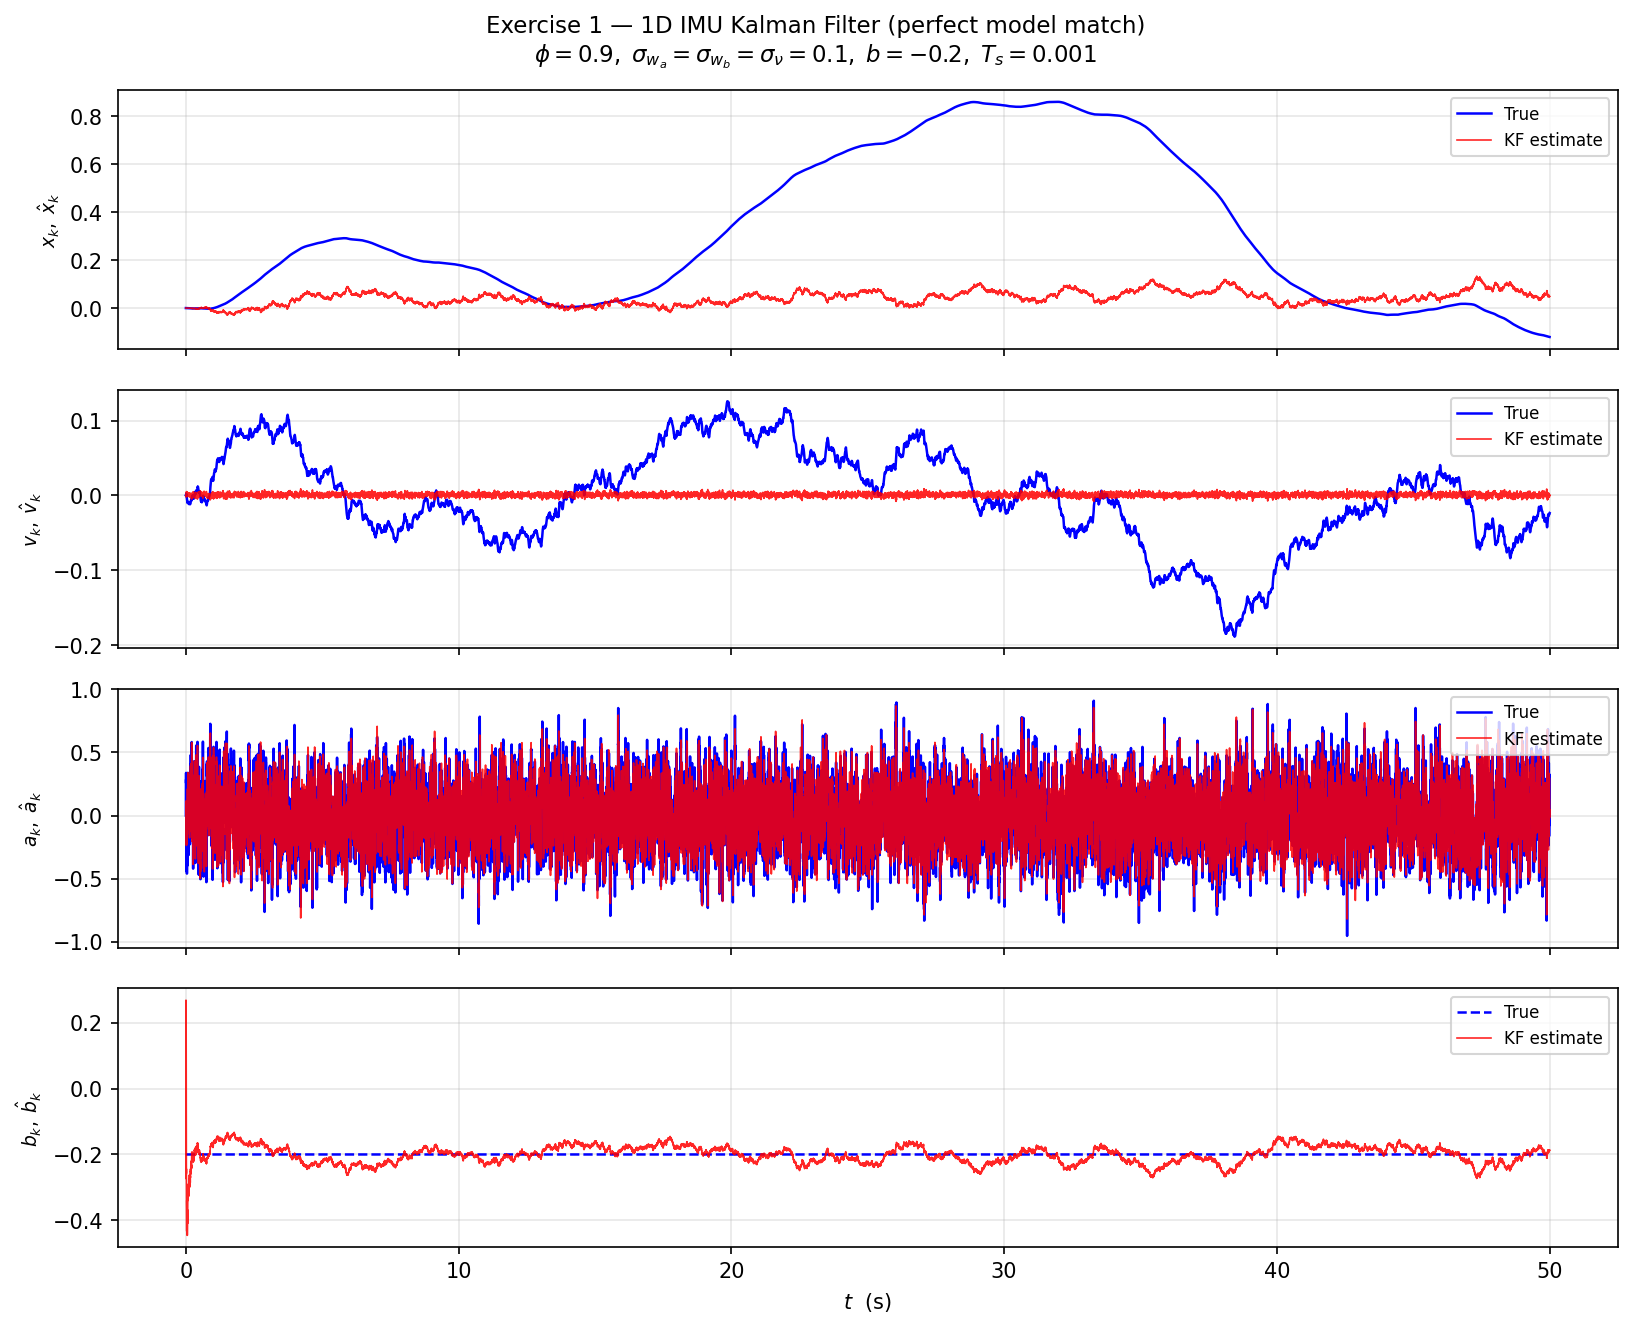
\includegraphics[width=0.7\linewidth]{../../Exercises/Lecture_5/exercise1_sigma_wb_0001.png}
  \caption{$\sigma_{w_b} = 0.001$: bias estimate hovers around $-0.2$
           with small persistent oscillations.
           Because $Q_{33} = 10^{-6} > 0$, the covariance prediction
           re-inflates $P^{[b,b]}$ every step, keeping $K^{[b]}$
           non-zero and preventing the estimate from locking in.}
  \label{fig:sigmawb0001}
\end{figure}
\begin{figure}[H]
  \centering
  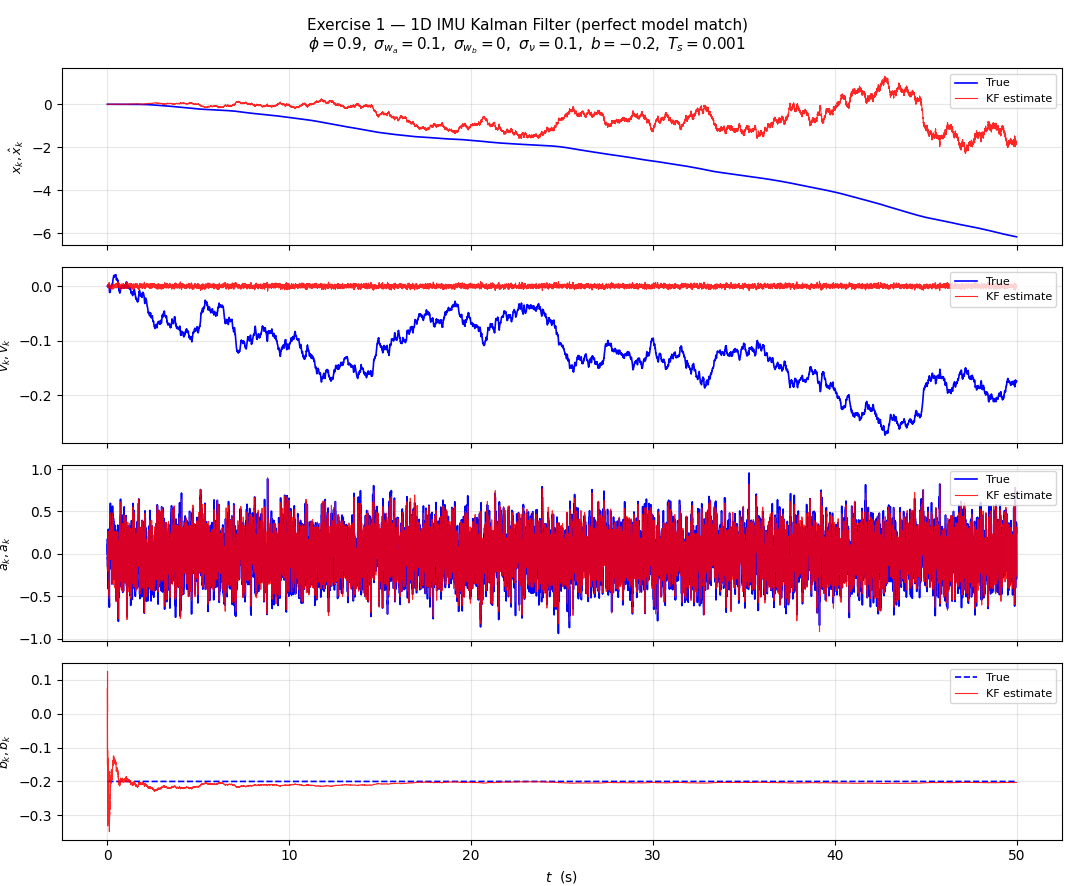
\includegraphics[width=0.7\linewidth]{../../Exercises/Lecture_5/omega_wb=0.00.PNG}
  \caption{Python simulation output.
           \textbf{Blue} = true signal; \textbf{Red} = KF estimate.
           Parameters: $\phi=0.9$, $\sigma_{w_a}=\sigma_\nu=0.0$,$\sigma_{w_b}=0.0$,
           $b=-0.2$, $T_s=0.001$, $N=50\,000$ steps (50\,s).}
  \label{fig:sigmawb00}
\end{figure}
\clearpage
\section*{Exercise 2 \quad Acceleration as External Input (Slide 27)}
Set acceleration as a known external input,
and combine it with the Kalman filter using the same parameter values.
Replicate the figures on Slide~27.
\vspace{-0.2cm}
\subsection*{Two-model approach}
\vspace{-0.2cm}
This exercise uses \textbf{two different models} running in parallel ---
one for the true physical system and one inside the Kalman filter.

\vspace{-0.2cm}
\subsection*{True system --- 3 states $[x,\,v,\,a]$:}
\vspace{-0.2cm}
\[
\underbrace{
\begin{bmatrix} x_{k+1} \\ v_{k+1} \\ a_{k+1} \end{bmatrix}
}_{\displaystyle\boldsymbol{\chi}_{\text{true},k+1}}
=
\underbrace{
\begin{bmatrix} 1 & T_s & 0 \\ 0 & 1 & T_s \\ 0 & 0 & 0 \end{bmatrix}
}_{\boldsymbol{\Phi}_{\text{true}},\;{\scriptsize\text{state transition}}}
\underbrace{
\begin{bmatrix} x_k \\ v_k \\ a_k \end{bmatrix}
}_{\displaystyle\boldsymbol{\chi}_{\text{true},k}}
+
\underbrace{
\begin{bmatrix} 0 \\ 0 \\ 1 \end{bmatrix}
}_{\displaystyle\boldsymbol{\Gamma}}
\underbrace{
a_k^{\text{input}}
}_{\scriptsize\text{known input}}
\quad
\begin{aligned}
  &\leftarrow x_{k+1} = x_k + T_s v_k\\
  &\leftarrow v_{k+1} = v_k + T_s a_k\\
  &\leftarrow a_{k+1} = a_k^{\text{input}}
\end{aligned}
\]
Acceleration is a \emph{known} deterministic input $a_k^{\text{input}}$, not a random state.
\vspace{-0.2cm}
\subsection*{Kalman filter --- 4 states $[x,\,v,\,a,\,b]$ (Slide~23/25 model):}
\vspace{-0.2cm}
The filter keeps 4 states with $\sigma_{w_b} = 0$ (bias fixed at $b = -0.2$, not a state in the true system --- a \textbf{model mismatch}).
The filter does \emph{not} know acceleration is sinusoidal; it uses the same AR(1) model with $\phi = 0.9$.
\vspace{-0.2cm}
\[
\underbrace{
\begin{bmatrix} x_{k+1} \\ v_{k+1} \\ a_{k+1} \\ b_{k+1} \end{bmatrix}
}_{\displaystyle\boldsymbol{\chi}_{k+1}}
=
\underbrace{
\begin{bmatrix}
  1 & T_s & 0    & 0 \\
  0 & 1   & T_s  & 0 \\
  0 & 0   & \phi & 0 \\
  0 & 0   & 0    & 1
\end{bmatrix}
}_{\boldsymbol{\Phi}_{\text{KF}},\;{\scriptsize\text{state transition}}}
\underbrace{
\begin{bmatrix} x_k \\ v_k \\ a_k \\ b_k \end{bmatrix}
}_{\displaystyle\boldsymbol{\chi}_k}
+
\underbrace{
\begin{bmatrix}
  0 & 0 & 0              & 0 \\
  0 & 0 & 0              & 0 \\
  0 & 0 & \sigma_{w_a}^2 & 0 \\
  0 & 0 & 0              & 0
\end{bmatrix}
}_{Q,\;{\scriptsize\text{process noise}}\;(\sigma_{w_b}=0)}^{1/2}
\underbrace{
\begin{bmatrix} 0 \\ 0 \\ \bar{w}_{a,k} \\ 0 \end{bmatrix}
}_{\displaystyle\bar{\mathbf{w}}_k}
\quad
\begin{aligned}
  &\leftarrow x_{k+1} = x_k + T_s v_k \quad \text{(Euler position)}\\
  &\leftarrow v_{k+1} = v_k + T_s a_k \quad \text{(Euler velocity)}\\
  &\leftarrow a_{k+1} = \phi\,a_k + \sigma_{w_a}\bar{w}_{a,k} \quad \text{(AR(1))}\\
  &\leftarrow b_{k+1} = b_k \quad \text{(bias fixed, no noise)}
\end{aligned}
\]
\vspace{-0.4cm}
\subsection*{Acceleration input, sum of two sinusoid}
\vspace{-0.1cm}
\[
  a_k^{\text{input}} = \sin(\omega_1 t) + 0.7\sin(\omega_2 t), \qquad
  \omega_1 = 2\pi\cdot 0.1\;\text{rad/s},\quad \omega_2 = 2\pi\cdot 1\;\text{rad/s}
\]

\begin{warnbox}
  \textbf{Model mismatch: sinusoidal input vs.\ AR(1) model.}\\
  The filter models acceleration as AR(1) with $\phi = 0.9$, giving a time constant
  $\tau = -T_s/\ln(\phi) \approx 10\,$ms --- meaning the \textbf{model expects acceleration
  to decorrelate in $\sim$10 steps}.
  
  The true input however contains a 0.1\,Hz component \textbf{correlated over thousands of steps}
  and a 1\,Hz component \textbf{correlated over hundreds}.

  The slow 0.1\,Hz sinusoid in particular resembles a drifting bias to the AR(1) filter
  --- it cannot distinguish a gradual rise/fall in acceleration from a shifting bias.
  Some sinusoidal variation therefore leaks into $\hat{b}$, causing the bias estimate
  to oscillate persistently around $-0.2$ rather than locking in.

  \textbf{Here the model mismatch is the source of the contamination.}
\end{warnbox}
\clearpage
\begin{figure}[H]
  \centering
  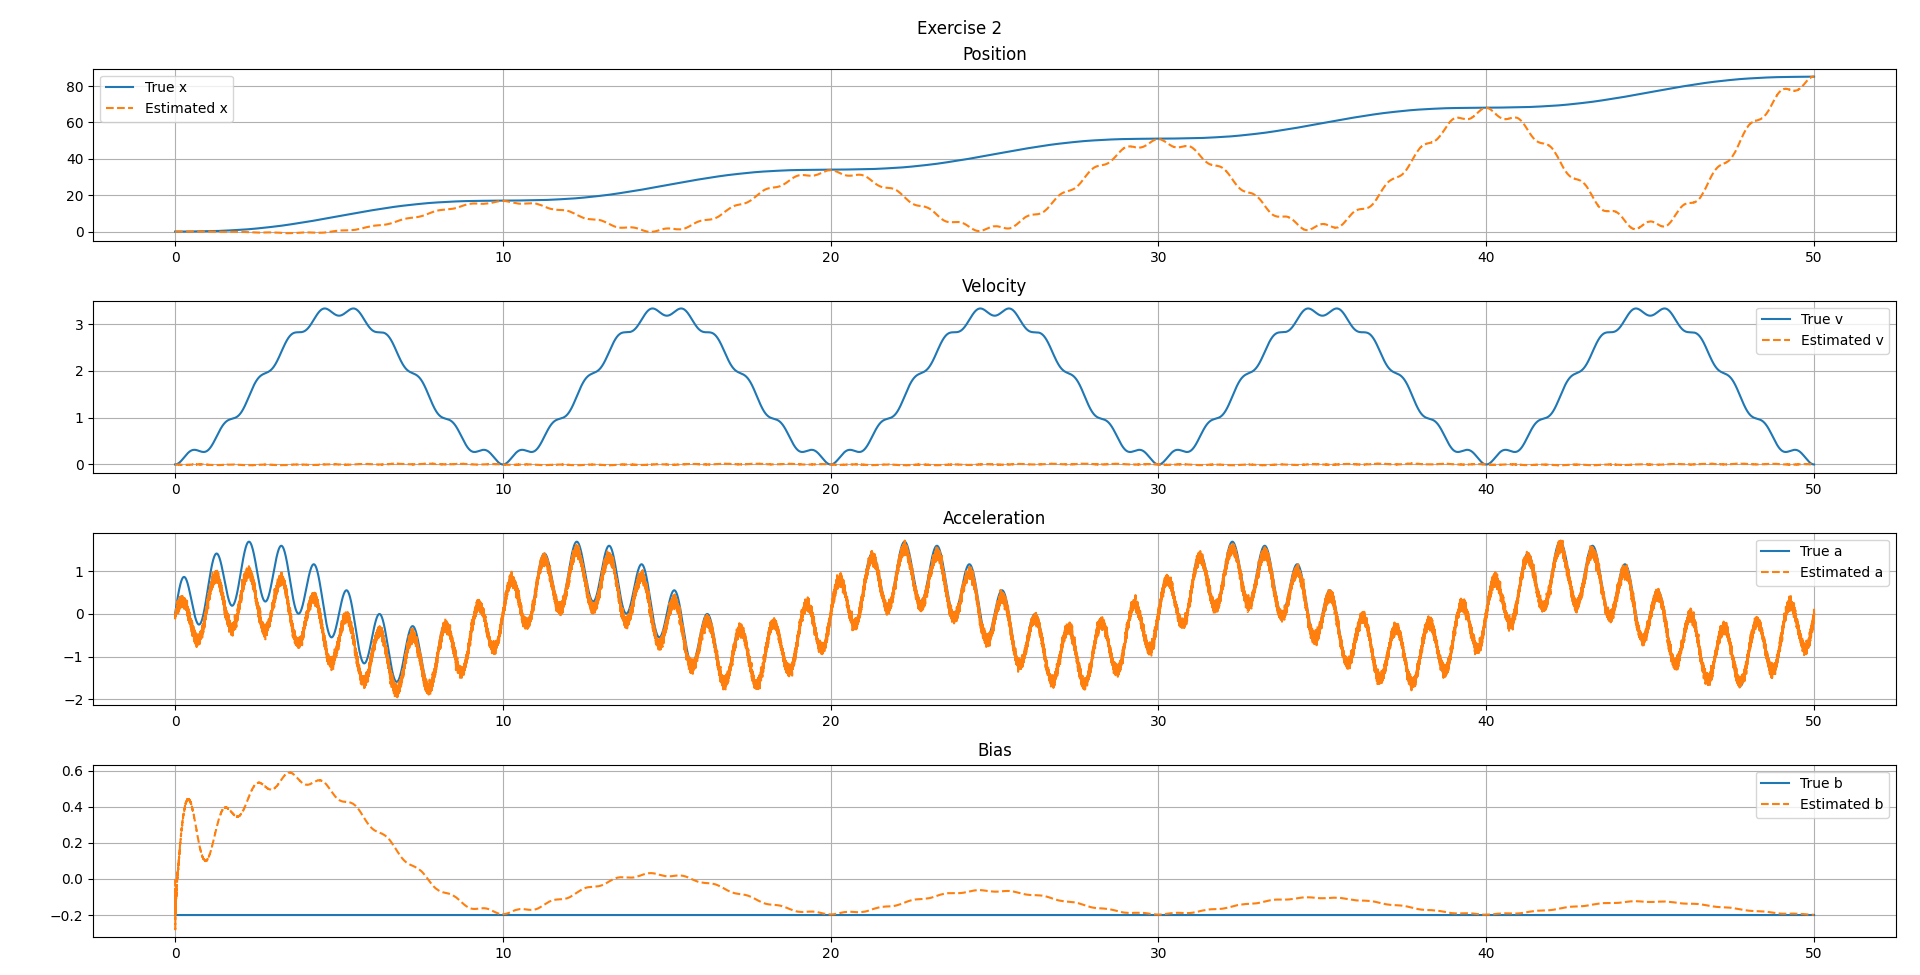
\includegraphics[width=0.7\linewidth]{../../Exercises/Lecture_5/exercise_2.png}
  \caption{Python simulation output.
           \textbf{Blue} = true signal; \textbf{Red} = KF estimate.
           Parameters: $\phi=0.9$, $\sigma_{w_a}=\sigma_\nu=0.1$, $\sigma_{w_b}=0.0$,
           $b=-0.2$, $T_s=0.001$, $N=50\,000$ steps (50\,s).}
  \label{fig:sigmawb00}
\end{figure}
\clearpage
\section*{Exercise 4 \quad Expand to 2D}
\vspace{-0.3cm}
Built on Exercise 2 with external acceleration input, now expanded to two independent axes.

\subsection*{True system --- 6 states $[x,\,v^x,\,a^x,\,y,\,v^y,\,a^y]$:}
\[
\underbrace{
\begin{bmatrix} x_{k+1} \\ v^x_{k+1} \\ a^x_{k+1} \\ y_{k+1} \\ v^y_{k+1} \\ a^y_{k+1} \end{bmatrix}
}_{\displaystyle\boldsymbol{\chi}_{\text{true},k+1}}
=
\underbrace{
\begin{bmatrix}
  1 & T_s & 0 & 0 & 0  & 0 \\
  0 & 1   & T_s & 0 & 0 & 0 \\
  0 & 0   & 0 & 0 & 0  & 0 \\
  0 & 0   & 0 & 1 & T_s & 0 \\
  0 & 0   & 0 & 0 & 1  & T_s \\
  0 & 0   & 0 & 0 & 0  & 0
\end{bmatrix}
}_{\boldsymbol{\Phi}_{\text{true}},\;{\scriptsize\text{state transition}}}
\underbrace{
\begin{bmatrix} x_k \\ v^x_k \\ a^x_k \\ y_k \\ v^y_k \\ a^y_k \end{bmatrix}
}_{\displaystyle\boldsymbol{\chi}_{\text{true},k}}
+
\underbrace{
\begin{bmatrix} 0 & 0 \\ 0 & 0 \\ 1 & 0 \\ 0 & 0 \\ 0 & 0 \\ 0 & 1 \end{bmatrix}
}_{\displaystyle\boldsymbol{\Gamma}}
\underbrace{
\begin{bmatrix} a^x_k \\ a^y_k \end{bmatrix}
}_{\scriptsize\text{known inputs}}
\quad
\begin{aligned}
  &\leftarrow x_{k+1}   = x_k + T_s v^x_k \\
  &\leftarrow v^x_{k+1} = v^x_k + T_s a^x_k \\
  &\leftarrow a^x_{k+1} = a^{x,\text{input}}_k \\
  &\leftarrow y_{k+1}   = y_k + T_s v^y_k \\
  &\leftarrow v^y_{k+1} = v^y_k + T_s a^y_k \\
  &\leftarrow a^y_{k+1} = a^{y,\text{input}}_k
\end{aligned}
\]
From $\boldsymbol{\Phi}_{\text{true}}$ it is clear that the two axes evolve independently ---
no cross-axis coupling. This is intentional: misalignment between axes is a
\textbf{deterministic} error (captured by $M_a$ in the full sensor model)
and is assumed to be calibrated away beforehand, not handled by the Kalman filter.

\subsection*{Kalman filter --- 8 states $[x,\,v^x,\,a^x,\,b^x,\,y,\,v^y,\,a^y,\,b^y]$:}
\textbf{Measurement equation:}
$y_k = H\,\boldsymbol{\chi}_k + R^{1/2}\bar{\nu}_k$
\vspace{-0.3cm}
\[
\underbrace{
\begin{bmatrix} x_{k+1} \\ v^x_{k+1} \\ a^x_{k+1} \\ b^x_{k+1} \\ y_{k+1} \\ v^y_{k+1} \\ a^y_{k+1} \\ b^y_{k+1} \end{bmatrix}
}_{\displaystyle\boldsymbol{\chi}_{k+1}}
=
\underbrace{
\begin{bmatrix}
  1 & T_s & 0   & 0 & 0 & 0  & 0   & 0 \\
  0 & 1   & T_s & 0 & 0 & 0  & 0   & 0 \\
  0 & 0   & \phi& 0 & 0 & 0  & 0   & 0 \\
  0 & 0   & 0   & 1 & 0 & 0  & 0   & 0 \\
  0 & 0   & 0   & 0 & 1 & T_s& 0   & 0 \\
  0 & 0   & 0   & 0 & 0 & 1  & T_s & 0 \\
  0 & 0   & 0   & 0 & 0 & 0  & \phi& 0 \\
  0 & 0   & 0   & 0 & 0 & 0  & 0   & 1
\end{bmatrix}
}_{\boldsymbol{\Phi}_{\text{KF}},\;{\scriptsize\text{state transtion}}}
\underbrace{
\begin{bmatrix} x_k \\ v^x_k \\ a^x_k \\ b^x_k \\ y_k \\ v^y_k \\ a^y_k \\ b^y_k \end{bmatrix}
}_{\displaystyle\boldsymbol{\chi}_k}
+
\underbrace{
\begin{bmatrix}
  0 & 0 & 0              & 0              & 0 & 0 & 0              & 0             \\
  0 & 0 & 0              & 0              & 0 & 0 & 0              & 0             \\
  0 & 0 & \sigma_{w_a^x}^2 & 0            & 0 & 0 & 0              & 0             \\
  0 & 0 & 0              & \sigma_{w_b^x}^2 & 0 & 0 & 0            & 0             \\
  0 & 0 & 0              & 0              & 0 & 0 & 0              & 0             \\
  0 & 0 & 0              & 0              & 0 & 0 & 0              & 0             \\
  0 & 0 & 0              & 0              & 0 & 0 & \sigma_{w_a^y}^2 & 0           \\
  0 & 0 & 0              & 0              & 0 & 0 & 0              & \sigma_{w_b^y}^2
\end{bmatrix}
}_{Q,\;{\scriptsize\text{process noise}}}^{1/2}
\underbrace{
\begin{bmatrix} 0 \\ 0 \\ \bar{w}^x_{a,k} \\ 0 \\ 0 \\ 0 \\ \bar{w}^y_{a,k} \\ 0 \end{bmatrix}
}_{\displaystyle\bar{\mathbf{w}}_k}
\]
\textbf{State equation:}
$\boldsymbol{\chi}_{k+1} = \boldsymbol{\Phi}\,\boldsymbol{\chi}_k + Q^{1/2}\bar{\mathbf{w}}_k$
Each row of $\boldsymbol{\Phi}$ encodes one update rule:
\[
\underbrace{
\begin{bmatrix} y^x_k \\ y^y_k \end{bmatrix}
}_{\displaystyle\mathbf{y}_k}
=
\underbrace{
\begin{bmatrix}
  0 & 0 & 1 & 1 & 0 & 0 & 0 & 0 \\
  0 & 0 & 0 & 0 & 0 & 0 & 1 & 1
\end{bmatrix}
}_{H,\;{\scriptsize\text{measurement matrix}}}
\underbrace{
\begin{bmatrix} x_k \\ v^x_k \\ a^x_k \\ b^x_k \\ y_k \\ v^y_k \\ a^y_k \\ b^y_k \end{bmatrix}
}_{\displaystyle\boldsymbol{\chi}_k}
+
\underbrace{
\begin{bmatrix} \sigma_{\nu^x}^2 & 0 \\ 0 & \sigma_{\nu^y}^2 \end{bmatrix}
}_{R,\;{\scriptsize\text{measurement noise}}}^{1/2}
\underbrace{
\begin{bmatrix} \bar{\nu}^x_k \\ \bar{\nu}^y_k \end{bmatrix}
}_{\displaystyle\bar{\boldsymbol{\nu}}_k}
\quad
\begin{aligned}
  &\leftarrow y^x_k = a^x_k + b^x_k + \sigma_{\nu^x}\bar{\nu}^x_k\\
  &\leftarrow y^y_k = a^y_k + b^y_k + \sigma_{\nu^y}\bar{\nu}^y_k
\end{aligned}
\]
Same assumes here also that two axes evolve independently ---
no cross-axis coupling. Calibrated away beforehand, not handled by the Kalman filter.

\begin{center}
\renewcommand{\arraystretch}{1.6}
\begin{tabular}{p{4.5cm} p{9.0cm}}
  \toprule
  \textbf{Syntax} & \textbf{What it does} \\
  \midrule
  \texttt{A @ B}
    & Matrix multiplication of \texttt{A} and \texttt{B}.
      Equivalent to \texttt{np.matmul(A, B)}.
      Works for 2-D arrays (matrix $\times$ matrix),
      2-D $\times$ 1-D (matrix $\times$ vector), and
      1-D $\times$ 1-D (dot product).
      Example: \texttt{H @ chi\_hat} multiplies the
      $(1\times4)$ matrix \texttt{H} by the $(4,)$ vector,
      giving a scalar. \\
  \texttt{np.eye(n)}
    & Returns the $n \times n$ \textbf{identity matrix} ---
      ones on the diagonal, zeros everywhere else.
      \texttt{np.eye(4)} gives the $4\times4$ identity used to
      initialise $P = I$ (``equal, moderate uncertainty in all
      states, no correlations''). \\
  \texttt{np.zeros(n)}
    & Returns a 1-D array of \texttt{n} zeros.
      \texttt{np.zeros(4)} gives \texttt{[0., 0., 0., 0.]} ---
      used to initialise \texttt{chi\_hat} (zero starting guess
      for all four states). \\
  \texttt{np.zeros(N)} (storage)
    & Same call, but used to pre-allocate an empty array of
      length $N$ to store results in the loop.
      Pre-allocating is faster than appending inside a loop. \\
  \texttt{np.diag([...])}
    & Creates a square \textbf{diagonal matrix} from a list.
      \texttt{np.diag([0, 0, 0.01, 0])} puts those values on
      the diagonal and zeros elsewhere --- used to build $Q$. \\
  \texttt{np.full(N, val)}
    & Returns an array of length $N$ where every entry is
      \texttt{val}.
      \texttt{np.full(N, -0.2)} creates the constant true-bias
      array for plotting. \\
  \texttt{np.random.randn()}
    & Draws \textbf{one} sample from $\mathcal{N}(0,1)$
      (standard normal: zero mean, unit variance). \\
  \texttt{np.random.randn(N)}
    & The argument \texttt{N} sets the \textbf{number of samples}
      returned --- gives a 1-D array of \texttt{N} independent
      draws from $\mathcal{N}(0,1)$.
      Used to generate all $N$ measurement noise samples at once
      rather than calling \texttt{randn()} inside the loop. \\
  \texttt{np.random.seed(s)}
    & Fixes the random number generator to seed \texttt{s} so
      the simulation produces the same random values every run.
      Remove or change \texttt{s} to get a different realization. \\
  \texttt{np.linalg.inv(A)}
    & Computes the \textbf{matrix inverse} $A^{-1}$.
      Used to compute $S_k^{-1}$ in the Kalman gain.
      For a scalar $S_k$ this is just $1/S_k$. \\
  \texttt{.flatten()}
    & Collapses any array to 1-D.
      After \texttt{K @ inn} the result can be shape $(4,1)$;
      \texttt{.flatten()} converts it to $(4,)$ so it can be
      added directly to \texttt{chi\_hat}. \\
  \texttt{.T}
    & \textbf{Transpose} of a 2-D array.
      \texttt{H.T} turns the $(1\times4)$ row vector into a
      $(4\times1)$ column vector. \\
  \bottomrule
\end{tabular}
\end{center}

\clearpage
\section*{Kalman Filter Equations --- Don't go say, don't think have time}
\vspace{-0.5cm}
\subsection*{Initialisation}
\vspace{-0.3cm}
\[
  \hat{\boldsymbol{\chi}}_{0|-1} = \mathbf{0}, \qquad P_{0|-1} = I
\]
$\hat{\boldsymbol{\chi}}_{0|-1} = \mathbf{0}$ is a neutral starting guess ---
all four states (position, velocity, acceleration, bias) set to zero
because we have no prior knowledge.

$P_{0|-1} = I$ sets the initial error covariance to the identity matrix.
The \textbf{diagonal entries of $P$ are the variances of each state estimate}

\begin{notebox}
  A larger diagonal entry means higher uncertainty (larger variance) for that state.
  Setting $P_{0|-1} = I$ is a moderate, equal initial guess:
  equal uncertainty across all four states and no assumed correlation between them
  (off-diagonal entries zero). Both values are overwritten rapidly once measurements arrive.
\end{notebox}

\subsection*{Step A --- Measurement update}
Runs every step as soon as a new sensor reading $y_k$ arrives.
The goal: correct the prediction from the previous step using
what the sensor just observed.

\textbf{1.\ Innovation}
\[
  \tilde{y}_{k|k-1} = y_k - H\hat{\boldsymbol{\chi}}_{k|k-1}
\]
could you add underbrace here to say predicted measurement under H and x

$y_k$ is a \textbf{scalar} --- a single accelerometer reading at step $k$.
This the acceleration measurement $y_k = a_k + b_k + \nu_k$. Not the True measurement
So true acceleration plus bias plus process/sensor noise

$\hat{\boldsymbol{\chi}}_{k|k-1}$ is the \textbf{predicted state} from the
previous step, a $4\times1$ vector $[\hat{x},\,\hat{v},\,\hat{a},\,\hat{b}]^\top$.

$H = [0,\,0,\,1,\,1]$ is the \textbf{measurement matrix}: it projects
the 4-state vector down to a scalar prediction of what the sensor
would read.

A large innovation means the measurement surprised the filter;
a small innovation means the prediction was already accurate.

\begin{notebox}
    $H$ come directly from the \textbf{sensor physics} ---
they are not a design choice.
For the accelerometer the physics says it reads exactly
$1{\cdot}a_k + 1{\cdot}b_k$, so the corresponding entries are 1 and 1.
The zeros for position and velocity are also physics: they genuinely
do not appear in what an accelerometer outputs.
\end{notebox}

\begin{defbox}
    $H\hat{\boldsymbol{\chi}}_{k|k-1}$ collapses the 4-state vector to a scalar:
$0{\cdot}\hat{x} + 0{\cdot}\hat{v} + 1{\cdot}\hat{a} + 1{\cdot}\hat{b}
= \hat{a}_{k|k-1} + \hat{b}_{k|k-1}$ ---
the filter's prediction of what the sensor would read.
\end{defbox}

\clearpage
\medskip
\textbf{2.\ Innovation covariance}
\[
  S_k = H\,P_{k|k-1}\,H^\top + R
\]

\begin{itemize}[leftmargin=1.4em, topsep=2pt]
  \item $H P_{k|k-1} H^\top$ --- the state prediction uncertainty
        \emph{projected into measurement space} via $H$.

        The $H$ matrices on each side extract only the
        acceleration/bias rows and columns of $P$, convertes state
        uncertainty into a scalar uncertainty.
    \item $R = \sigma_\nu^2$ --- the sensor noise variance; the
        irreducible noise on every individual reading.
\end{itemize}
Together they give the total uncertainty of the innovation, which
is used in the next step as a normalising denominator.

$S_k$ is the total variance of the innovation --- how uncertain we
should be about $\tilde{y}_{k|k-1}$ itself.

\medskip
\textbf{3.\ Kalman gain}
\[
  K_k = P_{k|k-1}\,H^\top\,S_k^{-1}
  \qquad\Longleftrightarrow\qquad
  K_k = \frac{\overbrace{P_{k|k-1}H^\top}^{\text{prediction uncertainty (in measurement space)}}}
             {\underbrace{S_k}_{\text{total uncertainty}}}
\]
$K_k$ is a $4\times1$ vector controlling how much each state is corrected by the innovation.
It is the \textbf{ratio of prediction uncertainty to total uncertainty}:
\begin{itemize}[leftmargin=1.4em]
  \item \textbf{Numerator} $P_{k|k-1}H^\top$: how uncertain the model prediction is, projected into measurement space.
  \item \textbf{Denominator} $S_k = HP_{k|k-1}H^\top + R$: that same prediction uncertainty plus sensor noise $R$.
\end{itemize}
A \textbf{high} $K_k$ means the model is uncertain relative to the sensor --- trust the measurement more.
A \textbf{low} $K_k$ means the sensor is noisy relative to the model --- trust the prediction more.

\begin{warnbox}
  In the general case $S_k \in \mathbb{R}^{m\times m}$ and $K_k \in \mathbb{R}^{n\times m}$,
  where $m$ is the number of measurements and $n$ the number of states.
  Here $y_k$ is a scalar (position only), so $m=1$ and $S_k$ collapses to a scalar.

  $P_{k|k-1}H^\top$ uses only $H^\top$ ($4\times1$), giving a $4\times1$ vector,
  whereas step 2. $S_k = HP_{k|k-1}H^\top + R$ sandwiches with both $H$ and $H^\top$,
  which collapses the result to a scalar.

  Therefore $K_k = (4\times1)/(1\times1)$ remains a $4\times1$ vector --- one gain per state.
\end{warnbox}
\textbf{4.\ State update}
\[
  \hat{\boldsymbol{\chi}}_{k|k} = \hat{\boldsymbol{\chi}}_{k|k-1} + K_k\,\tilde{y}_{k|k-1}
\]
$\hat{\boldsymbol{\chi}}_{k|k-1}$ is the prediction (built from all data up
to step $k-1$).

The result $\hat{\boldsymbol{\chi}}_{k|k}$ is now the best estimate
at step $k$ after having seen $y_k$ --- \textbf{uncertainty decreases}.

\textbf{5.\ Covariance update (Joseph form)}
\[
  P_{k|k} = (I - K_k H)\,P_{k|k-1}\,(I - K_k H)^\top + K_k R K_k^\top
\]

After seeing the measurement, the filter knows more about the state,
so $P$ shrinks --- \textbf{uncertainty decreases}.

The factor $(I - K_k H)$ represents how much uncertainty is
\emph{not} explained by the measurement: if $K_k H = I$ (perfect
observation of all states) the whole prior uncertainty is cancelled.

The extra $K_k R K_k^\top$ adds back the small residual uncertainty
introduced by the sensor noise itself.

\begin{notebox}
    The symmetric sandwich form $(I-K_kH)\,P\,(I-K_kH)^\top$ is used
instead of the simpler $(I-K_kH)P$ because it keeps $P$ symmetric
and positive-definite even after thousands of steps of floating-point
arithmetic --- a numerical stability guarantee.
\end{notebox}

\subsection*{Step B --- Time update (prediction)}
Runs immediately after Step~A to prepare the estimate for the next step.

\medskip
\textbf{1.\ State prediction}
\[
  \hat{\boldsymbol{\chi}}_{k+1|k} = \boldsymbol{\Phi}\,\hat{\boldsymbol{\chi}}_{k|k}
\]
$\boldsymbol{\Phi}$ is the \textbf{model's approximation} of how the
true system evolves --- it is not the exact true transition, just the
best mathematical description.

Multiplying the corrected estimate $\hat{\boldsymbol{\chi}}_{k|k}$ by $\boldsymbol{\Phi}$ rolls it
one step forward. The output $\hat{\boldsymbol{\chi}}_{k+1|k}$ is the predicted state
for the next step, ready to be corrected again when $y_{k+1}$ arrives.

\medskip
\textbf{2.\ Covariance prediction}
\[
  P_{k+1|k} = \boldsymbol{\Phi}\,P_{k|k}\,\boldsymbol{\Phi}^\top + Q
\]

$\boldsymbol{\Phi}\,P_{k|k}\,\boldsymbol{\Phi}^\top$ propagates the
current uncertainty forward through the dynamics model --- the same way
$\boldsymbol{\Phi}$ propagates the state estimate.

$Q$ is then \textbf{added} on top.
It is the noise process noise --- it is the covariance of the random
\textbf{kick} each state takes during the transition itself.

$Q = \mathrm{diag}(0,\,0,\,\sigma_{w_a}^2,\,\sigma_{w_b}^2)$ is the
covariance matrix of those kicks --- it describes \emph{how wide the
distribution of the next state is} given the current one, not anything
a sensor reads.

The larger $Q$ is, the more the filter admits it does not know exactly
where the state will land next step, and the faster $P$ grows.

\textbf{uncertainty grows} during prediction and is only brought back
down when the next measurement arrives in Step~A.





\clearpage
\begin{notebox}
\textbf{Worked example for $HPH^\top$} with $H=[0,0,1,1]$ and a
concrete $P$. {\color{keyblue}Blue} marks the rows $H$ picks from $P$;
{\color{warnred}red} marks the columns $H^\top$ picks from $HP$.

\[
P =
\begin{bmatrix}
  0.5 & 0   & 0   & 0   \\
  0   & 0.4 & 0   & 0   \\
  {\color{keyblue}0} & {\color{keyblue}0} & {\color{keyblue}0.3} & {\color{keyblue}0.1} \\
  {\color{keyblue}0} & {\color{keyblue}0} & {\color{keyblue}0.1} & {\color{keyblue}0.2}
\end{bmatrix}
\]

\textbf{Step 1 --- $HP$:} $[0,0,1,1]$ multiplies $P$, adding
{\color{keyblue}row~3} $+$ {\color{keyblue}row~4}:
\[
  HP = \bigl[0{+}0,\;\; 0{+}0,\;\;
       {\color{warnred}0.3{+}0.1},\;\;
       {\color{warnred}0.1{+}0.2}\bigr]
     = \bigl[0,\;0,\;{\color{warnred}0.4},\;{\color{warnred}0.3}\bigr]
\]

\textbf{Step 2 --- $(HP)H^\top$:} dot with $[0,0,1,1]^\top$, picking
{\color{warnred}columns~3 and~4} of $HP$:
\[
  HPH^\top
  = 0{\cdot}0 + 0{\cdot}0
    + {\color{warnred}0.4}{\cdot}1
    + {\color{warnred}0.3}{\cdot}1
  = 0.7
\]

So the result is the sum of the \textbf{four entries in the
$a$--$b$ corner of $P$}:
\[
  HPH^\top
  = \underbrace{P_{33}}_{0.3}
  + \underbrace{P_{34}}_{0.1}
  + \underbrace{P_{43}}_{0.1}
  + \underbrace{P_{44}}_{0.2}
  = 0.7
\]

The combined uncertainty about $a+b$ is larger than adding their variances alone.
The position and velocity rows/columns vanish entirely because of
the zeros in $H$ --- their uncertainty is irrelevant to what the
accelerometer reads.
\end{notebox}





\end{document}



